\subsection{Eigenvalues and Eigenvectors}

\begin{definition}{Eigenvalue and Eigenvector}{eigen}
  Let $\mathbf{A} \in \R^{n \times n}$. A vector $\mathbf{v} \in \R^n$ is an \textbf{eigenvector} of $\mathbf{A}$ with \textbf{eigenvalue} $\lambda \in \R$ if
  \begin{enumerate}
    \item $\mathbf{v} \neq \mathbf{0}$, and
    \item $\mathbf{A}\mathbf{v} = \lambda \mathbf{v}$.
  \end{enumerate}
\end{definition}

\begin{example}
  Let $\mathbf{A} =
    \begin{bmatrix}
      2 & 1 \\ 1 & 2
    \end{bmatrix}
  $. Is $\mathbf{v} = \ve{2, 3}$ an eigenvector? Compute
  \[
    \mathbf{A}\mathbf{v} =
    \begin{bmatrix}
      2 & 1 \\ 1 & 2
    \end{bmatrix}
    \begin{bmatrix}
      2 \\ 3
    \end{bmatrix}
    =
    \begin{bmatrix}
      7 \\ 8
    \end{bmatrix}
    ,
  \]
  which is not a scalar multiple of $\ve{2, 3}$, so $\mathbf{v}$ is not an eigenvector.
\end{example}

\subsubsection{Geometric Meaning}

Identify $\mathbf{A}$ with the linear map $T(\mathbf{x}) = \mathbf{A}\mathbf{x}$. An eigenvector $\mathbf{v}$ is a direction preserved by $T$: $T(\mathbf{v})$ lies on the same line through the origin as $\mathbf{v}$, scaled by $\lambda$.

\begin{center}
  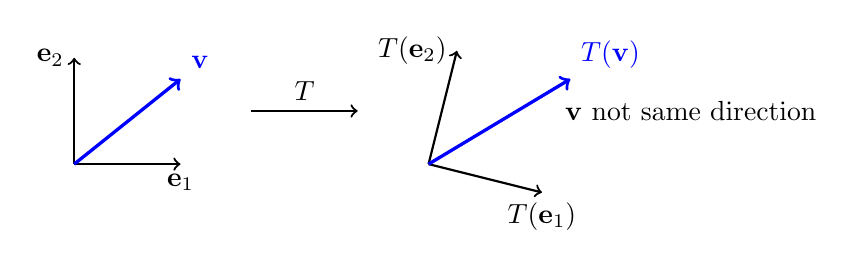
\begin{tikzpicture}[scale=0.9]
    \begin{scope}
      \draw[->, thick] (0,0) -- (1.5,0) node[below] {$\mathbf{e}_1$};
      \draw[->, thick] (0,0) -- (0,1.5) node[left] {$\mathbf{e}_2$};
      \draw[->, very thick, blue] (0,0) -- (1.5,1.2) node[above right] {$\mathbf{v}$};
    \end{scope}
    \draw[->, thick] (2.5,0.75) -- (4,0.75) node[midway, above] {$T$};
    \begin{scope}[xshift=5cm]
      \draw[->, thick] (0,0) -- (1.6,-0.4) node[below] {$T(\mathbf{e}_1)$};
      \draw[->, thick] (0,0) -- (0.4,1.6) node[left] {$T(\mathbf{e}_2)$};
      \draw[->, very thick, blue] (0,0) -- (2.0,1.2) node[above right] {$T(\mathbf{v})$};
    \end{scope}
    \node at (8.7,0.75) {$\mathbf{v}$ not same direction};
  \end{tikzpicture}
\end{center}

\subsubsection{Finding Eigenvalues}

Rearranging $\mathbf{A}\mathbf{v} = \lambda \mathbf{v}$ with $\mathbf{v} \neq \mathbf{0}$:
\[
  \mathbf{A}\mathbf{v} = \lambda \mathbf{I} \mathbf{v}
  \iff (\mathbf{A} - \lambda \mathbf{I})\mathbf{v} = \mathbf{0}.
\]
Since this homogeneous system has a non-trivial solution, $\mathbf{A} - \lambda \mathbf{I}$ must be singular:
\[
  \det(\mathbf{A} - \lambda \mathbf{I}) = 0.
\]

\begin{definition}{Characteristic Equation}{characteristic-eq}
  The eigenvalues of $\mathbf{A} \in \R^{n \times n}$ are the roots of the \textbf{characteristic equation}
  \[
    \det(\mathbf{A} - \lambda \mathbf{I}) = 0.
  \]
\end{definition}

\begin{example}
  Find the eigenvalues and eigenvectors of $\mathbf{A} =
    \begin{bmatrix}
      2 & 1 \\ 1 & 2
    \end{bmatrix}
  $.

  \medskip

  \emph{Eigenvalues.}
  \[
    \mathbf{A} - \lambda \mathbf{I} =
    \begin{bmatrix}
      2 - \lambda & 1           \\
      1           & 2 - \lambda
    \end{bmatrix}
    ,
    \quad
    \det(\mathbf{A} - \lambda \mathbf{I}) = (2 - \lambda)^2 - 1 = 0.
  \]
  Solving, $(2 - \lambda)^2 = 1$ gives $\lambda_1 = 3$, $\lambda_2 = 1$.

  \medskip

  \emph{Eigenvector for $\lambda_1 = 3$.} Solve $(\mathbf{A} - 3\mathbf{I})\mathbf{v} = \mathbf{0}$:
  \[
    \begin{bmatrix}
      -1 & 1  \\
      1  & -1
    \end{bmatrix}
    \mathbf{v}_1 = \mathbf{0}
    \implies \{\mathbf{v}_1\} = \operatorname{span}\left\{
    \begin{bmatrix}
      1 \\ 1
    \end{bmatrix}
    \right\}
    .
  \]

  \emph{Eigenvector for $\lambda_2 = 1$.} Solve $(\mathbf{A} - \mathbf{I})\mathbf{v}_2 = \mathbf{0}$:
  \[
    \begin{bmatrix}
      1 & 1 \\
      1 & 1
    \end{bmatrix}
    \mathbf{v}_2 = \mathbf{0}
    \implies \{\mathbf{v}_2\} = \operatorname{span}\left\{
    \begin{bmatrix}
      1 \\ -1
    \end{bmatrix}
    \right\}
    .
  \]
\end{example}

\subsection{Eigenbasis}

\begin{definition}{Eigenbasis}{eigenbasis}
  Let $\mathbf{A} \in \R^{n \times n}$. An \textbf{eigenbasis} for $\R^n$ is a basis $\beta = \{\mathbf{v}_1, \ldots, \mathbf{v}_n\}$ whose every vector is an eigenvector of $\mathbf{A}$:
  \[
    \operatorname{span}(\beta) = \R^n,
    \quad
    \mathbf{A}\mathbf{v}_j = \lambda_j \mathbf{v}_j \text{ for } j \in \{1, \ldots, n\}.
  \]
\end{definition}

\begin{remark}
  Spanning $\R^n$ with $n$ vectors already forces $\mathbf{v}_1, \ldots, \mathbf{v}_n$ to be linearly independent, so no separate check is needed.
\end{remark}

\begin{example}
  Continuing $\mathbf{A} =
    \begin{bmatrix}
      2 & 1 \\ 1 & 2
    \end{bmatrix}
  $ from the previous example, the eigenvectors
  \[
    \mathbf{v}_1 =
    \begin{bmatrix}
      1 \\ 1
    \end{bmatrix}
    ,
    \quad
    \mathbf{v}_2 =
    \begin{bmatrix}
      1 \\ -1
    \end{bmatrix}
  \]
  span $\R^2$, so $\beta = \{\mathbf{v}_1, \mathbf{v}_2\}$ is an eigenbasis.
\end{example}

\subsection{Diagonalization}

\begin{definition}{Diagonal Matrix}{diag-matrix}
  A \textbf{diagonal matrix} has nonzero entries only on its main diagonal:
  \[
    \mathbf{D} =
    \begin{bmatrix}
      \lambda_1 &        & 0         \\
                & \ddots &           \\
      0         &        & \lambda_n
    \end{bmatrix}
    .
  \]
\end{definition}

The eigenvalues of $\mathbf{D}$ are exactly its diagonal entries:
\[
  \det(\mathbf{D} - \lambda \mathbf{I}) =
  \det
  \begin{bmatrix}
    \lambda_1 - \lambda &        & 0                   \\
                        & \ddots &                     \\
    0                   &        & \lambda_n - \lambda
  \end{bmatrix}
  = \prod_{i=1}^{n} (\lambda_i - \lambda),
\]
so $\lambda = \lambda_1, \ldots, \lambda_n$.

\begin{definition}{Diagonalizable Matrix}{diagonalizable}
  $\mathbf{A} \in \R^{n \times n}$ is \textbf{diagonalizable} if there exist a diagonal $\mathbf{D} \in \R^{n \times n}$ and an invertible $\mathbf{P} \in \R^{n \times n}$ such that
  \[
    \mathbf{P}^{-1} \mathbf{A} \mathbf{P} = \mathbf{D}.
  \]
\end{definition}

\begin{remark}
  The columns of $\mathbf{P}$ form an eigenbasis for $\mathbf{A}$. Left-multiplying $\mathbf{P}^{-1}\mathbf{A}\mathbf{P} = \mathbf{D}$ by $\mathbf{P}$ gives $\mathbf{A}\mathbf{P} = \mathbf{P}\mathbf{D}$. Writing $\mathbf{P} = [\mathbf{v}_1 \mid \cdots \mid \mathbf{v}_n]$,
  \[
    [\mathbf{A}\mathbf{v}_1 \mid \cdots \mid \mathbf{A}\mathbf{v}_n]
    = [\lambda_1 \mathbf{v}_1 \mid \cdots \mid \lambda_n \mathbf{v}_n],
  \]
  so $\mathbf{A}\mathbf{v}_j = \lambda_j \mathbf{v}_j$ for each $j$.
\end{remark}

\begin{theorem}{Diagonalizability Criterion}{diagonalizable-iff}
  $\mathbf{A} \in \R^{n \times n}$ is diagonalizable iff there exist $n$ linearly independent eigenvectors $\mathbf{v}_1, \ldots, \mathbf{v}_n$ of $\mathbf{A}$. In that case
  \[
    \mathbf{P} = [\mathbf{v}_1 \mid \cdots \mid \mathbf{v}_n],
    \quad
    \mathbf{D} =
    \begin{bmatrix}
      \lambda_1 &        & 0         \\
                & \ddots &           \\
      0         &        & \lambda_n
    \end{bmatrix}
    .
  \]
\end{theorem}

\begin{remark}[Eigenbasis language]
  The essence of diagonalization is rewriting vectors in the \emph{eigenbasis language}. Given an eigenbasis $\beta = \{\mathbf{v}_1, \ldots, \mathbf{v}_n\}$, any $\mathbf{x} \in \R^n$ has a unique expansion $\mathbf{x} = c_1 \mathbf{v}_1 + \cdots + c_n \mathbf{v}_n$, with coordinate vector $[\mathbf{x}]_\beta = \mathbf{P}^{-1}\mathbf{x}$. In this new language $\mathbf{A}$ acts as the diagonal matrix $\mathbf{D}$:
  \[
    \mathbf{A}\mathbf{x} = c_1 \lambda_1 \mathbf{v}_1 + \cdots + c_n \lambda_n \mathbf{v}_n
    \implies [\mathbf{A}\mathbf{x}]_\beta = \mathbf{D}\,[\mathbf{x}]_\beta,
  \]
  which is exactly the statement $\mathbf{P}^{-1}\mathbf{A}\mathbf{P} = \mathbf{D}$.
\end{remark}

\begin{example}
  Is $\mathbf{A} =
    \begin{bmatrix}
      2 & 1 \\ 1 & 2
    \end{bmatrix}
  $ diagonalizable? From the previous example, $\lambda_1 = 3$ and $\lambda_2 = 1$ with eigenvectors
  \[
    \begin{bmatrix}
      1 \\ 1
    \end{bmatrix}
    \text{ at } \lambda_1,
    \quad
    \begin{bmatrix}
      1 \\ -1
    \end{bmatrix}
    \text{ at } \lambda_2.
  \]
  These are linearly independent, so $\beta = \left\{
    \begin{bmatrix}
      1 \\ 1
    \end{bmatrix}
    ,
    \begin{bmatrix}
      1 \\ -1
    \end{bmatrix}
    \right\}$ is an eigenbasis and
  \[
    \mathbf{P} =
    \begin{bmatrix}
      1 & 1  \\
      1 & -1
    \end{bmatrix}
    ,
    \quad
    \mathbf{D} =
    \begin{bmatrix}
      3 & 0 \\
      0 & 1
    \end{bmatrix}
    .
  \]
\end{example}

\begin{example}
  Find the eigenvalues of $\mathbf{A} =
    \begin{bmatrix}
      6 & 7 \\ 6 & 7
    \end{bmatrix}
  $.
  \[
    \det(\mathbf{A} - \lambda \mathbf{I}) = (6 - \lambda)(7 - \lambda) - 42 = \lambda^2 - 13\lambda = 0,
  \]
  so $\lambda_1 = 0$ and $\lambda_2 = 13$.
  \begin{remark}
    $\lambda = 0$ is an eigenvalue of $\mathbf{A}$ $\iff$ $\mathbf{A}$ is non-invertible.
  \end{remark}
\end{example}

\begin{theorem}{Independence from Distinct Eigenvalues}{distinct-eigvals-indep}
  Eigenvectors of $\mathbf{A}$ corresponding to distinct eigenvalues are linearly independent.
\end{theorem}
